\chapter{Mechanik}

\renewcommand{\kapitelautor}{Autor: Alexander Punz}

\section{Rotorschutz}
In dem gewählten Bausatz des Hexacopters ist kein Rotorschutz beinhaltet, eines der Zeile ist es den Rotor möglichst gut zu schützen und das maximale Abfluggewicht nicht zu überschreiten. Da der Hexacopter mit einer maximalen Last von 1,9 kg belastet werden kann, können Materialen wie Stahl oder Aluminium für den Rotorschutz nicht verwendet werden. 
Da die Möglichkeit besteht, Teile in einer vernünftigen Qualität vor Ort drucken zu können, wurde die Fertigung mittels des 3D-Druckers gewählt. Mit diesem ist es möglich den erforderlichen Rotorschutz sehr genau und leicht drucken zu können. 
Die folgende Abbildung zeigt den fertigen Rotorschutz.

\begin{figure}[tbh]
\begin{centering}
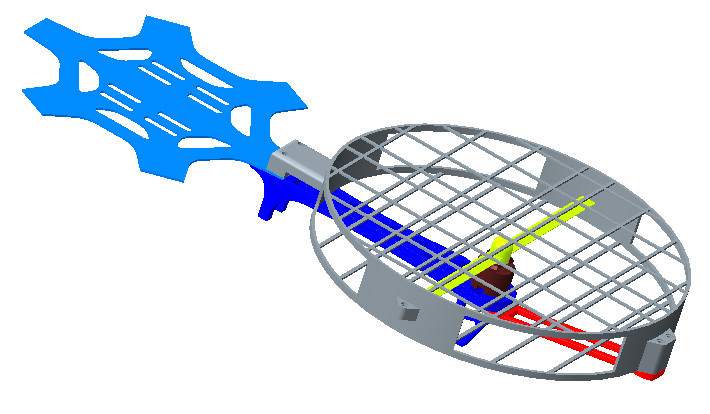
\includegraphics[width = 100mm]{Bilder/rotorschutz_zusammenbau}
\par\end{centering}
\caption{Rotorschutz systematisch dargestellt}
\label{Rotorschutz}
\end{figure}

Der Rotorschutz umrandet den Propeller, damit dieser im Falle eines Absturzes nicht zerstört wird. Die Lamellen ober- und unterhalb des Rotors sollen Personen gegen Verletzungen schützen. 
Der Ring wird durch die Strebe (rot) gestützt, damit er nicht nach unten abbrechen kann. 
Durch die großen Abmessungen bzw. der Form, kann der Ring nicht als ein Teil gedruckt werden, er wird dadurch in verschiedene Sektoren unterteilt. Der Ring wird in eine untere und obere Hälfte unterteilt bzw. beide Hälften wieder in zwei Teile. Die einzelnen Glieder werden dann mit Schrauben und Zweikomponentenkleber zusammengefügt. 

\section{Halterung des Ultraschallsensors}
An dem Hexacopter wird ein Ultraschallsensor angebracht, der die Höhe des Copters messen soll, das ist wichtig damit dieser in der richtigen Höhe fliegt. Der Sensor wird mittels einer selbst konstruierten und angefertigten Halterung am Multicopter montiert.
Bei der Konstruktion der Halterung ist es wichtig, dass sie so leicht wie möglich bzw. einfach anzubringen ist. Die folgenden Abbildungen zeigen die Position bzw. die angefertigte Halltevorrichtung.

\begin{figure}[htb]
\begin{centering}
\includegraphics[width = 100mm]{Bilder/halterung_ultraschall_creo}
\par\end{centering}
\caption{Position der Halterung am Hexacopter}
\label{Halterung des Ultraschallsensor}
\end{figure}

\begin{figure}[htb]
\begin{centering}
\includegraphics[width = 60mm]{Bilder/halterung_ultraschall_fertig}
\par\end{centering}
\caption{angefertigte Halterung des Ultraschallsensor}
\label{Halterung des Ultraschallsensor}
\end{figure}

Die Halterung wurde, wie auch der Rotorschutz, im 3D Drucker angefertigt, da das Material sehr leicht ist und die Form sehr einfach anzufertigen ist. Mittels den drei Laschen, wird das Werkstück an der Centerplate angeklammert.
Das Material ist so robust, dass man diese weit auseinander dehnen, aber sie sich dann wieder zurückverformen können. 


